\section{Xác thực đối tượng người dùng}
\subsection{Cơ chế xác thực}
\section{Chức năng từng đối tượng trong hệ thống}
Từ việc thiết kế Usecase ở chương 4, nhóm nghiên cứu tiến hành thực hiện từng chức năng tương ứng với mỗi đối tượng. Cụ thể từng chức năng quan trọng như sau:
\subsection{Đối tượng: Quản trị hệ thống}
\textbf{Chức năng: Cấu hình cho hệ thống}
\begin{center}
  \captionsetup{type=figure}
  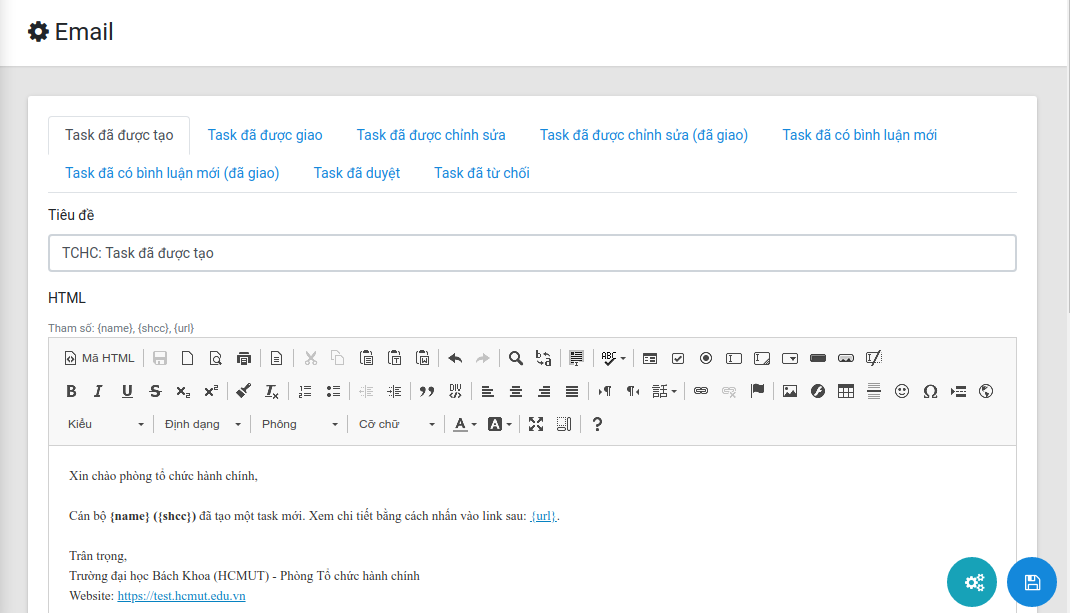
\includegraphics[scale=0.5]{img/Screen/email.png}
  \captionof{figure}{Cấu hình Email cho hệ thống}
\end{center}
Phần này giúp quản trị viên thực hiện việc \textbf{soạn thảo nội dung} của email và nội dung của email này sẽ được sử dụng ở nhiều mục đích khác nhau. Trong nội dung của email, hệ thống có cung cấp những \textbf{tham số} cho quản trị viên sử dụng khi cần thiết. Các tham số này sẽ được thay thế bằng những từ phù hợp bởi hệ thống trước khi gửi đi cho người dùng.\\
\textbf{Chức năng: Quản lý tài khoản người dùng}\\
 - Lược đồ Activity:
 \begin{center}
  \captionsetup{type=figure}
  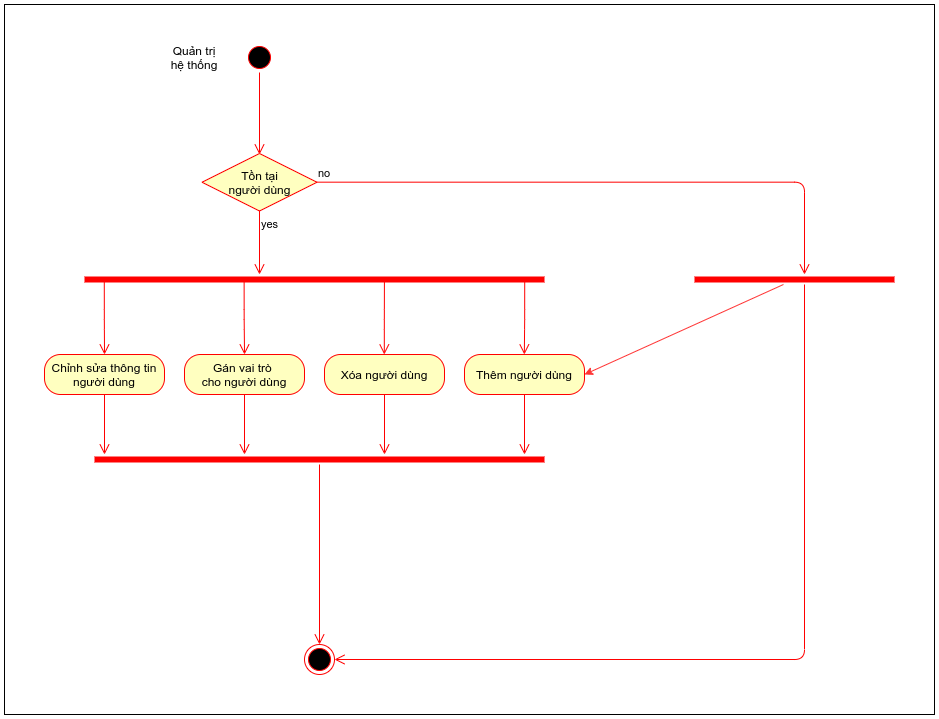
\includegraphics[scale=0.5]{img/UML/Admin/addUserActivity.png}
  \captionof{figure}{Lược đồ Activity quản lý tài khoản người dùng}
\end{center}
\begin{center}
  \captionsetup{type=figure}
  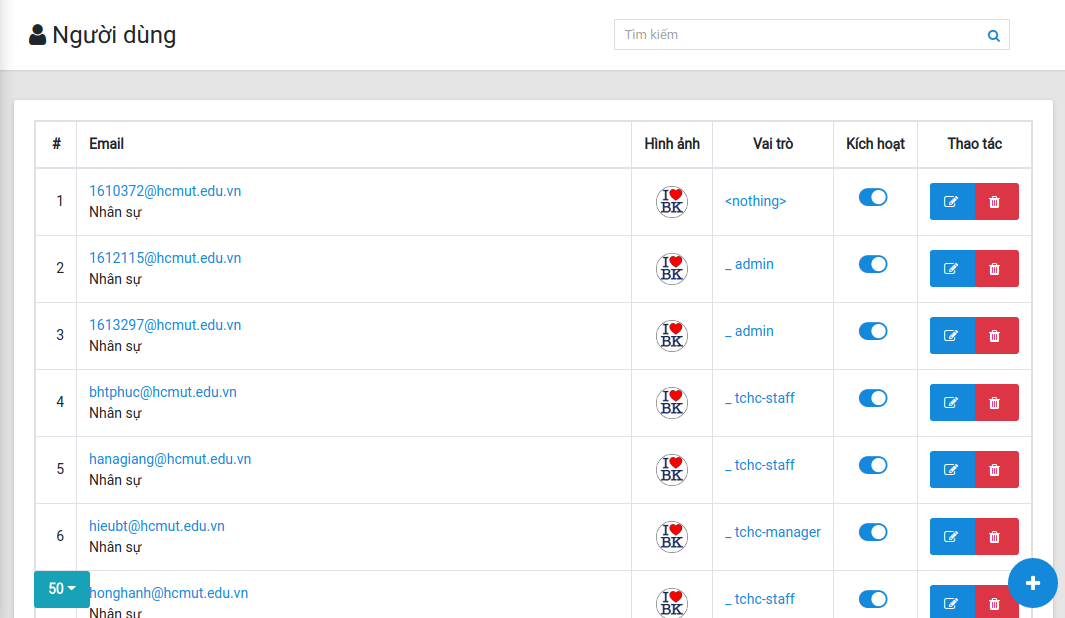
\includegraphics[scale=0.5]{img/Screen/user.png}
  \captionof{figure}{Danh sách người dùng hiện có của hệ thống}
\end{center}

Phần này giúp quản trị viên quản lý được người dùng trong hệ thống. Quản trị viên có thêm xem danh xóa toàn bộ người dùng, chỉnh sửa các thông tin của từng người dùng, đặt vai trò trong hệ thống, xóa người dùng ra khỏi hệ thống.\\
\begin{center}
  \captionsetup{type=figure}
  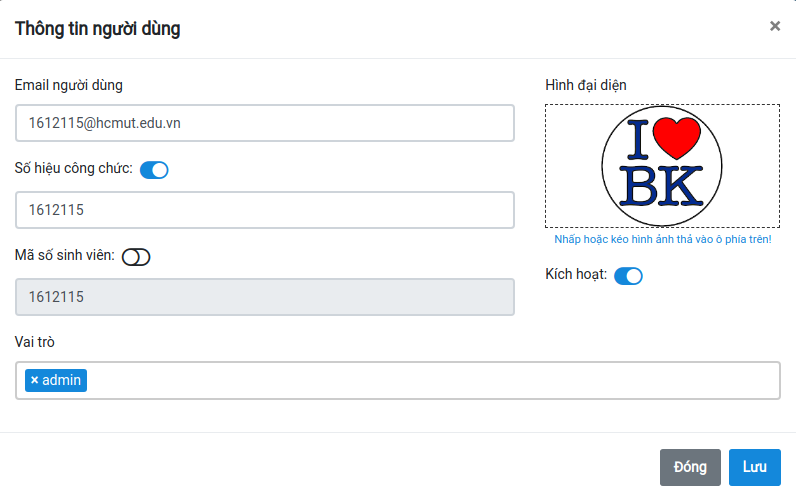
\includegraphics[scale=0.6]{img/Screen/editUser.png}
  \captionof{figure}{Chỉnh sửa thông tin người dùng}
\end{center}
\textbf{Chức năng: Quản lý vai trò trong hệ thống}\\
- Lược đồ Activity:
\begin{center}
  \captionsetup{type=figure}
  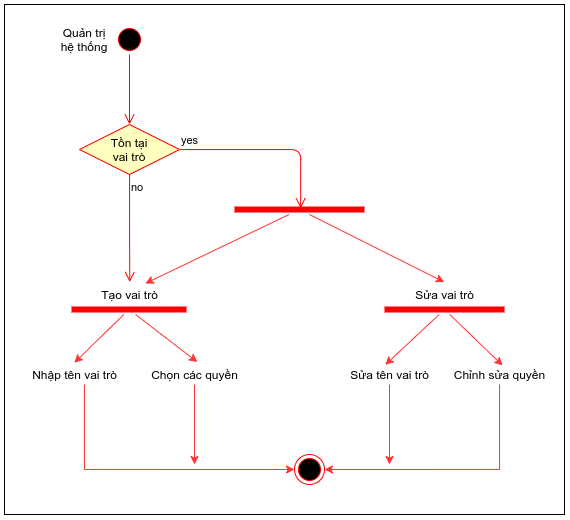
\includegraphics[scale=0.6]{img/UML/Admin/addRole.png}
  \captionof{figure}{Lược đồ Activity quản lý vai trò hệ thống}
\end{center}
- Đặc tả: Chức năng này cho phép người quản trị hệ thống thêm vai trò mới vào hệ thống và gán quyền cho vai trò.\\
- Lược đồ sequence:\\
- Hình ảnh mình họa:
\begin{center}
  \captionsetup{type=figure}
  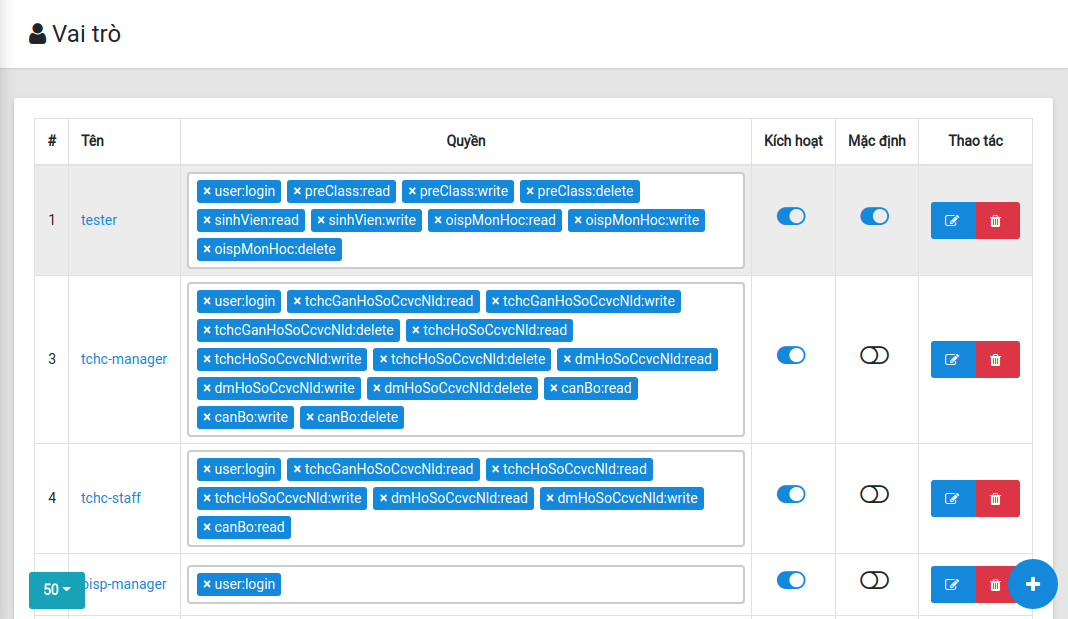
\includegraphics[scale=0.6]{img/Screen/allrole.png}
  \captionof{figure}{Danh sách vai trò có trong hệ thống hiện tại}
\end{center}
\textbf{Chức năng: Quản lý trang chủ}
\begin{center}
  \captionsetup{type=figure}
  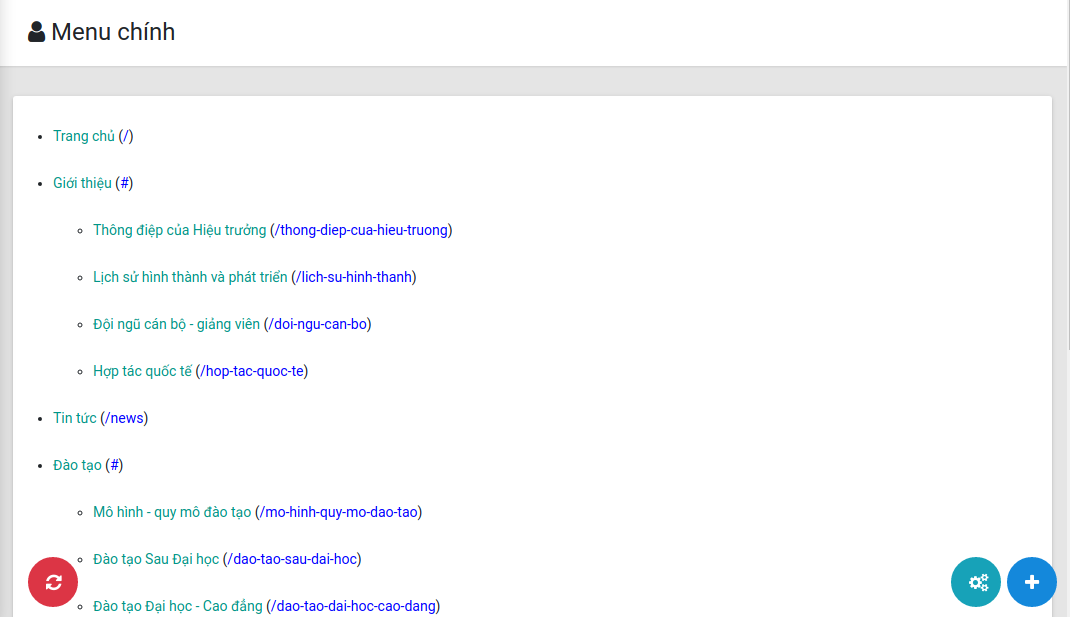
\includegraphics[scale=0.6]{img/Screen/menu.png}
  \captionof{figure}{Danh sách menu của trang}
\end{center}

Phần này giúp quản trị viên thiết kế phần menu header của trang chủ như là: tạo mới menu kèm theo đường dẫn, kích hoạt menu, thay đổi thứ tự hiển thị.\\

\textbf{Chức năng: Cấu hình các Section trong một trang giao diện cụ thể}
\begin{center}
  \captionsetup{type=figure}
  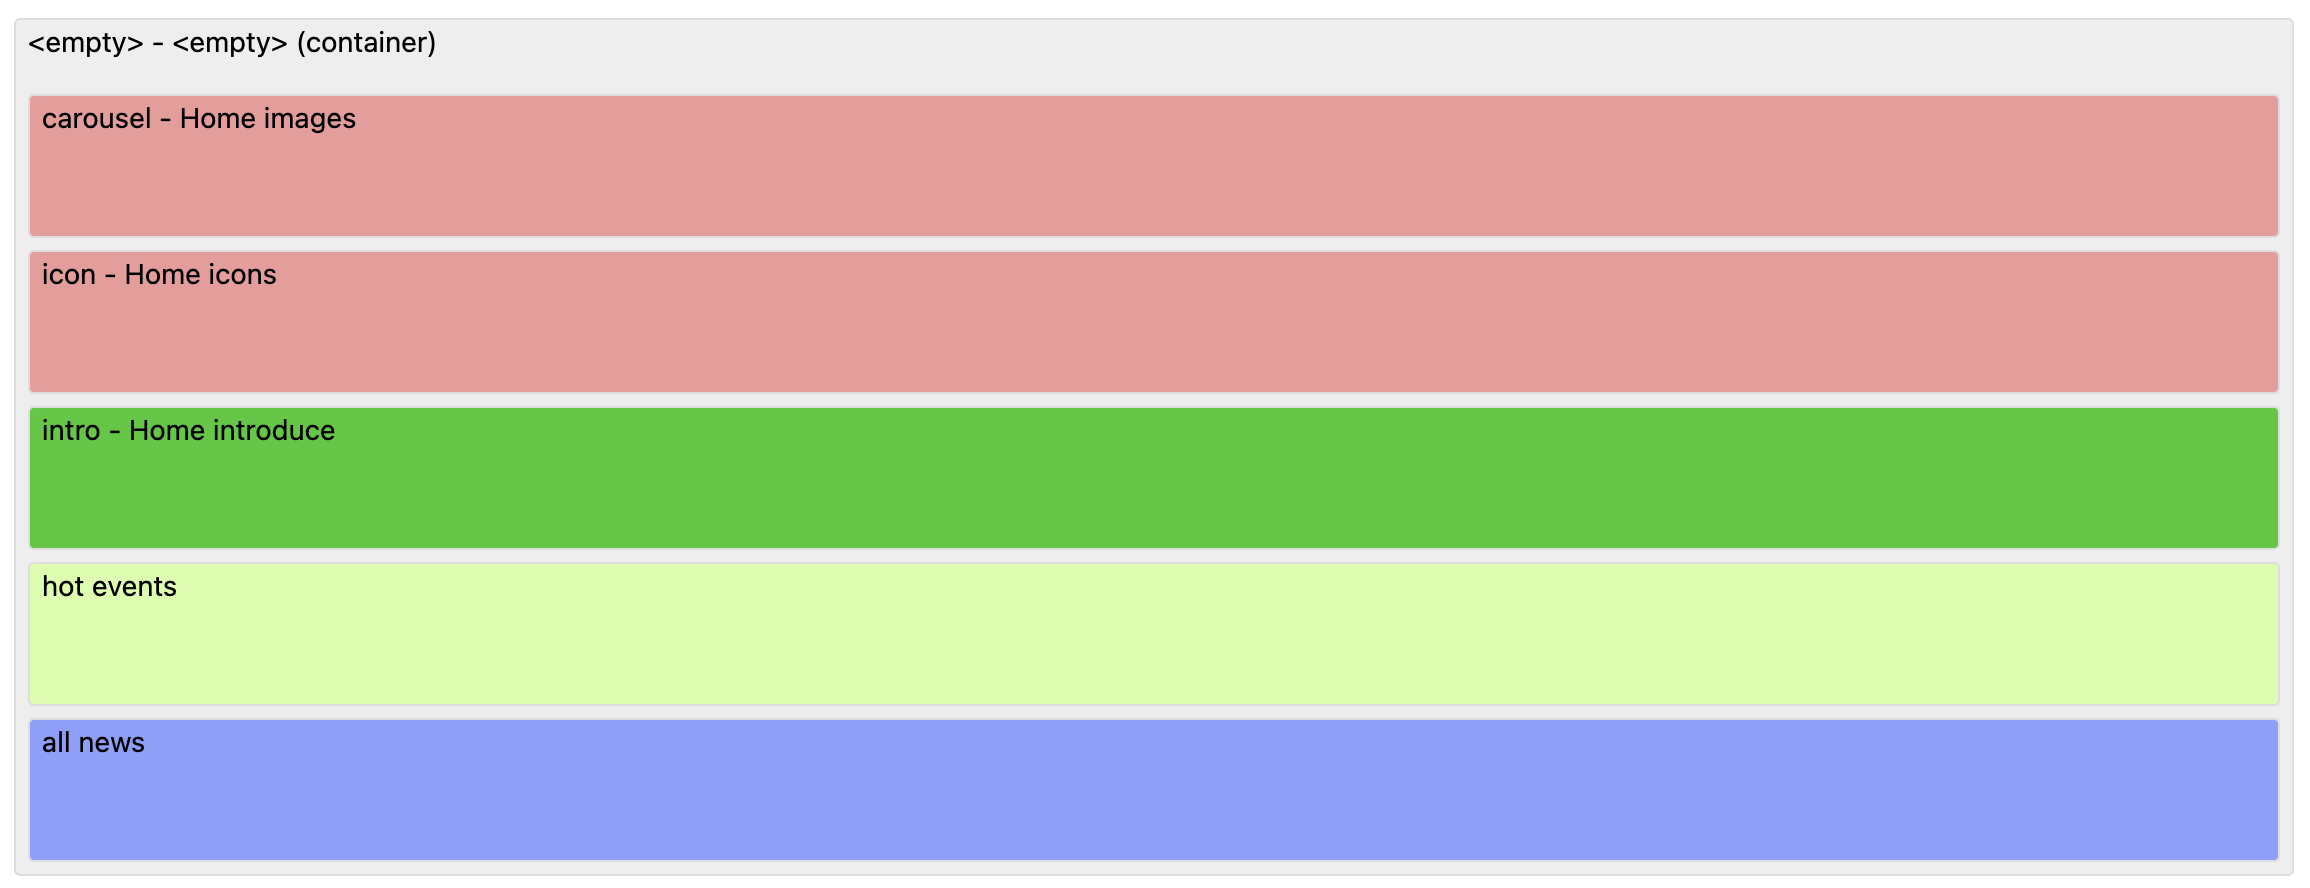
\includegraphics[scale=0.6]{img/Screen/section.png}
  \captionof{figure}{Danh sách section của một trang giao diện cụ thể}
\end{center}

Ở một trang chủ cụ thể, quản trị viên có thể thiết lập trang đó gồm những thành phần nào và thứ tự xuất hiện của các thành phần đó.\\
\textbf{Chức năng: Quản lý thông tin danh mục}\\
- Lược đồ Activity đối với từng danh mục
\begin{center}
  \captionsetup{type=figure}
  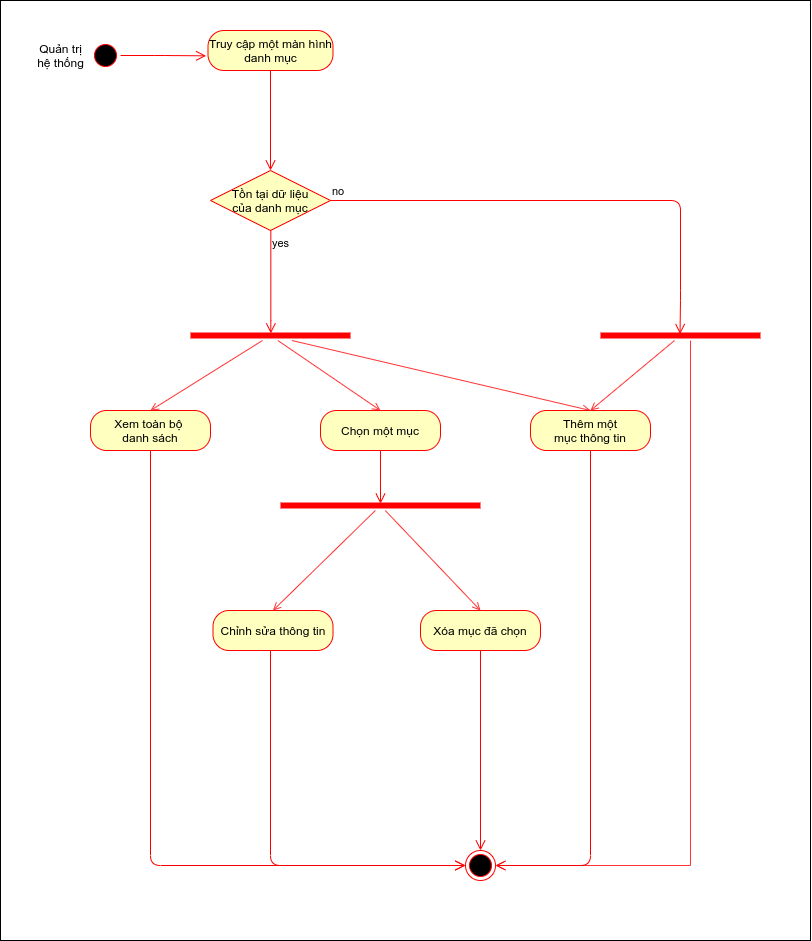
\includegraphics[scale=0.7]{img/UML/Admin/danhmucActivity.png}
  \captionof{figure}{Lược đồ Activity quản lý danh mục}
\end{center}
\subsection{Đối tượng: Trưởng phòng và cán bộ phòng Tổ chức - Hành chính}
\textbf{Chức năng: Gán hồ sơ cho cán bộ}\\
- Lược đồ Activity:
\begin{center}
  \captionsetup{type=figure}
  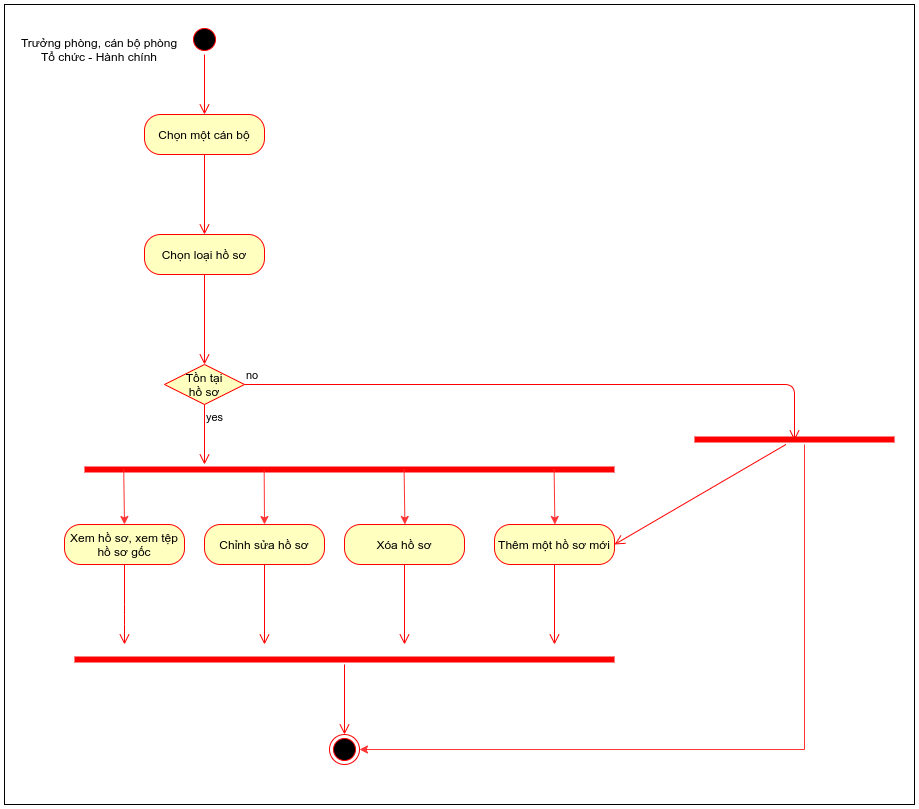
\includegraphics[scale=0.5]{img/UML/Manager/activityQuanLyHoSo.png}
  \captionof{figure}{Lược đồ Activity quản lý hồ sơ cán bộ}
\end{center}
- Đặc tả: Chức năng cho phép quản lý các hồ sơ của cán bộ. Lưu trữ hồ sơ gốc dưới dạng tệp trên hệ thống.\\
- Lược đồ Sequence: \\
- Hình ảnh cụ thể: 
\begin{center}
  \captionsetup{type=figure}
  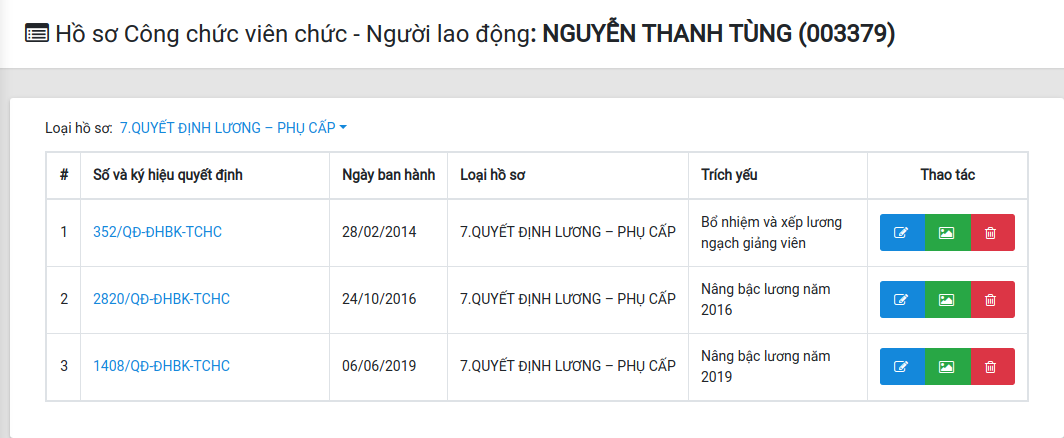
\includegraphics[scale=0.5]{img/Screen/qlhoso.png}
  \captionof{figure}{Quản lý hồ sơ cán của cán bộ}
\end{center}
\textbf{Chức năng: Quản lý cán bộ}\\
- Lược đồ Activity:
\begin{center}
  \captionsetup{type=figure}
  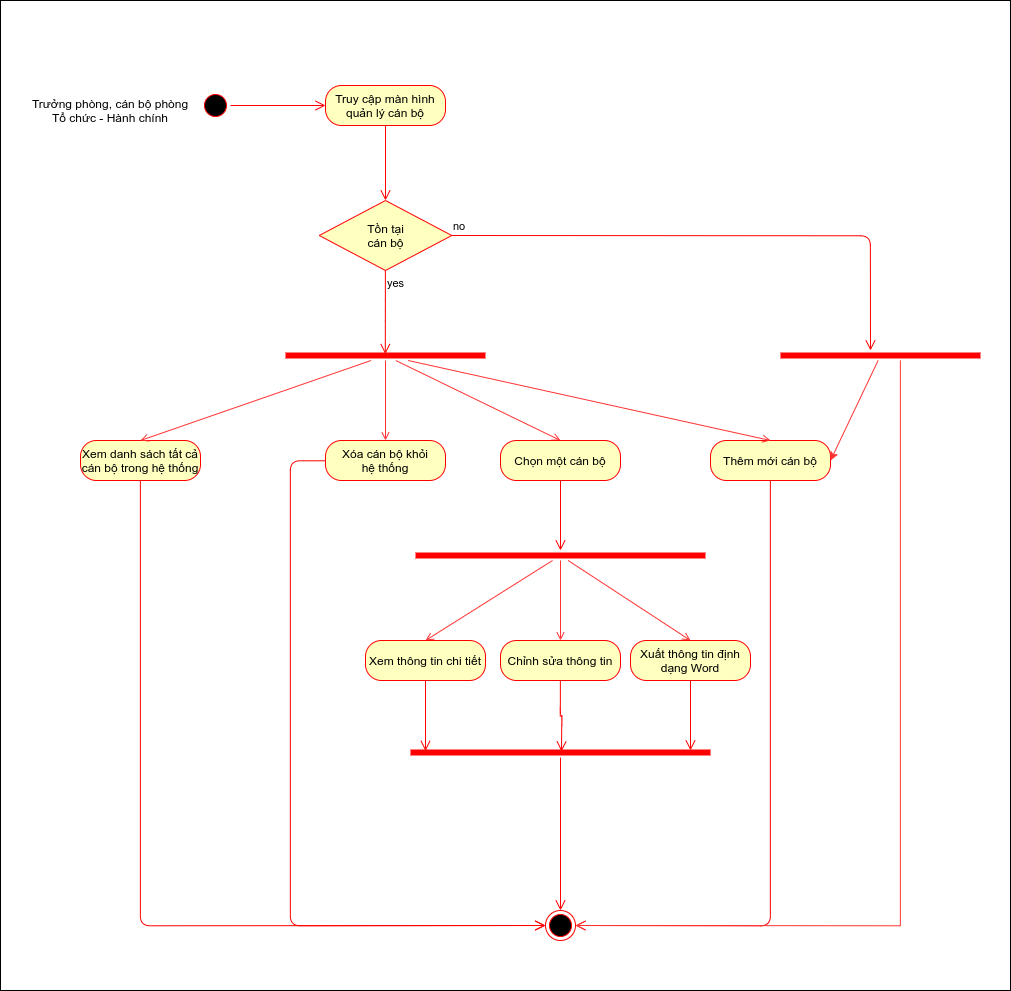
\includegraphics[scale=0.4]{img/UML/TchcStaff/activityQuanLyCanBo.png}
  \captionof{figure}{Lược đồ Activity chức năng quản lý thông tin cán bộ}
\end{center}
- Đặc tả: Đây là chức năng cho phép đối tượng là cán bộ phòng Tổ chức - Hành chính có thể xem và chỉnh sửa thông tin của toàn bộ cán bộ hiện có trong hệ thống, thêm cán bộ vào hệ thống, xóa cán bộ khỏi hệ thống. Bên cạnh đó họ còn có thể xuất thông tin của cán bộ ra tệp tin Word theo mẫu của Bộ nội vụ.\\
- Lược đồ Sequence:\\
- Hình ảnh chi tiết:
\begin{center}
  \captionsetup{type=figure}
  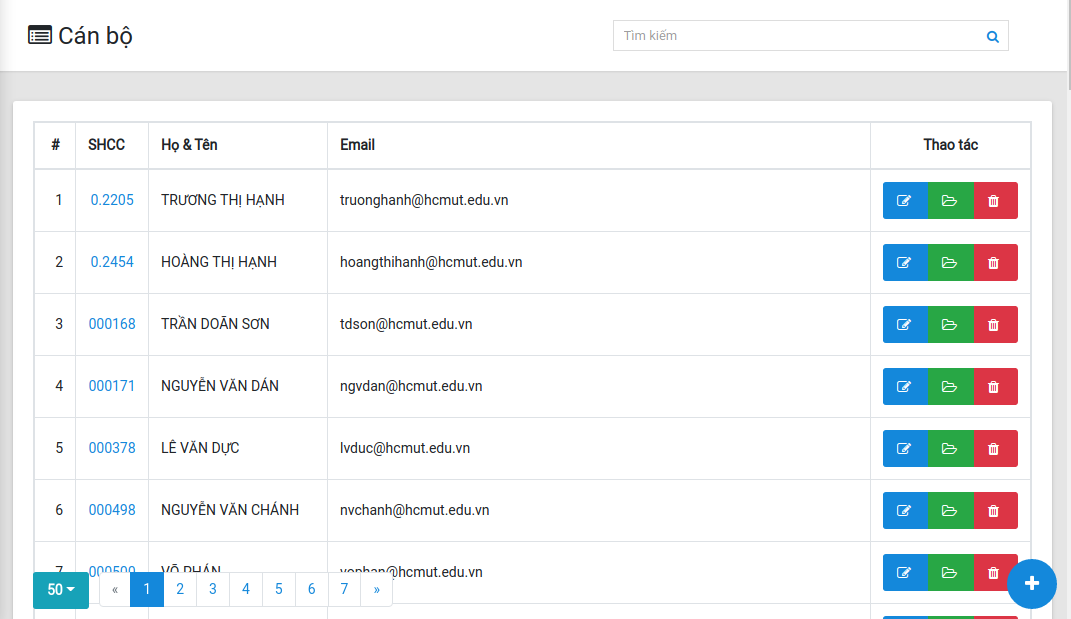
\includegraphics[scale=0.5]{img/Screen/allcanbo.png}
  \captionof{figure}{Danh sách toàn bộ cán bộ}
\end{center}
\begin{center}
  \captionsetup{type=figure}
  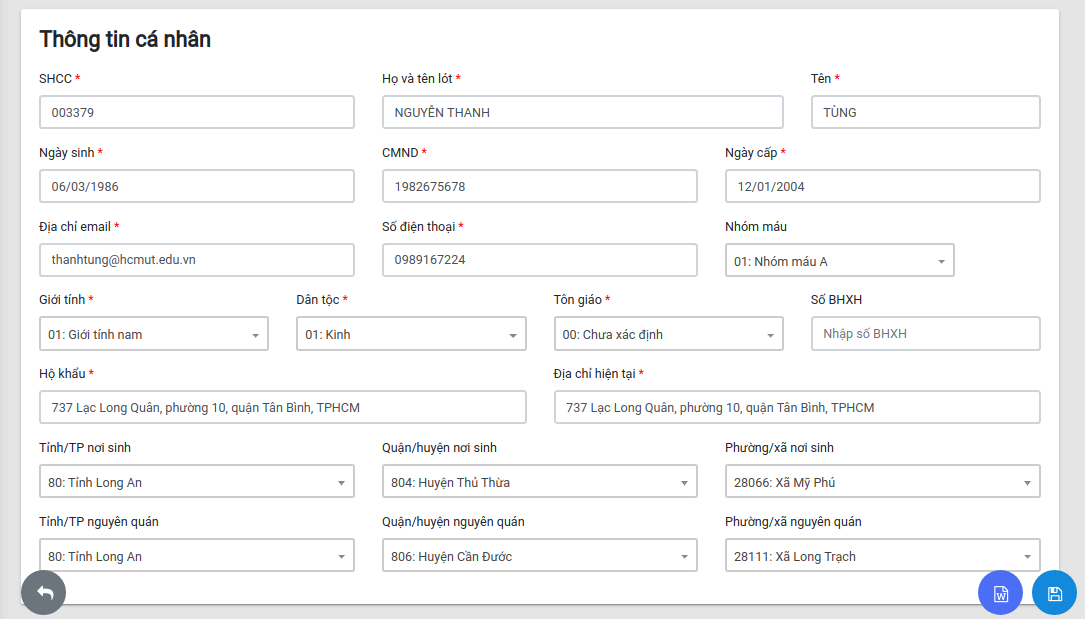
\includegraphics[scale=0.5]{img/Screen/edithongtin.png}
  \captionof{figure}{Xem, chỉnh sửa thông tin cán bộ}
\end{center}
\textbf{Chức năng: Quản lý đối với một quá trình nghiệp vụ}\\
- Lược đồ Activity:
\begin{center}
  \captionsetup{type=figure}
  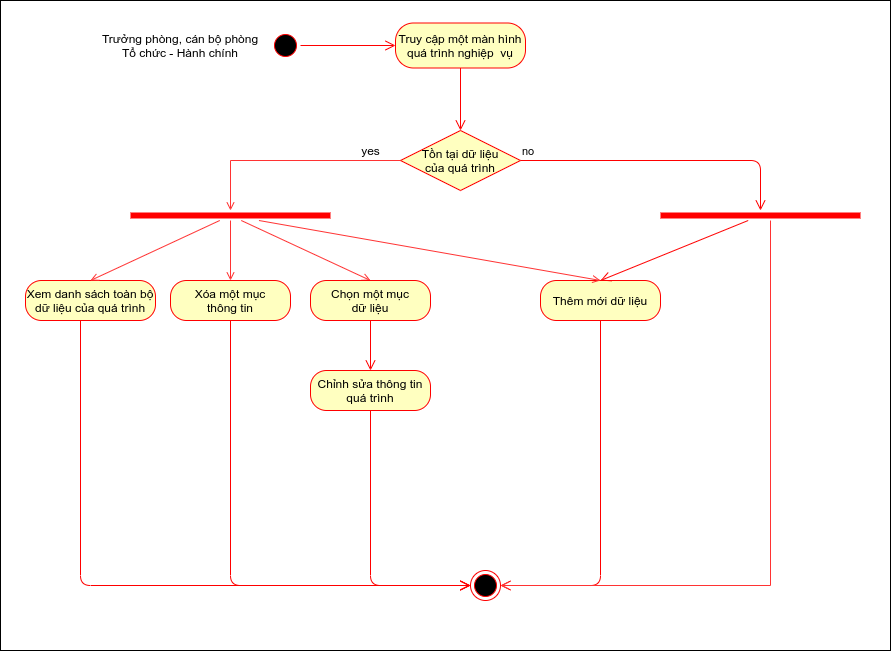
\includegraphics[scale=0.5]{img/UML/TchcStaff/activityQuanLyQT.png}
  \captionof{figure}{Lược đồ Activity quản lý quá trình nghiệp vụ}
\end{center}
- Đặc tả: Chức năng này cho phép cán bộ phòng Tổ chức - Hành chính quản lý các quá trình nghiệp vụ của cán bộ trong trường.\\
- Lược đồ Sequence: \\
- Hình ảnh chi tiết:
\begin{center}
  \captionsetup{type=figure}
  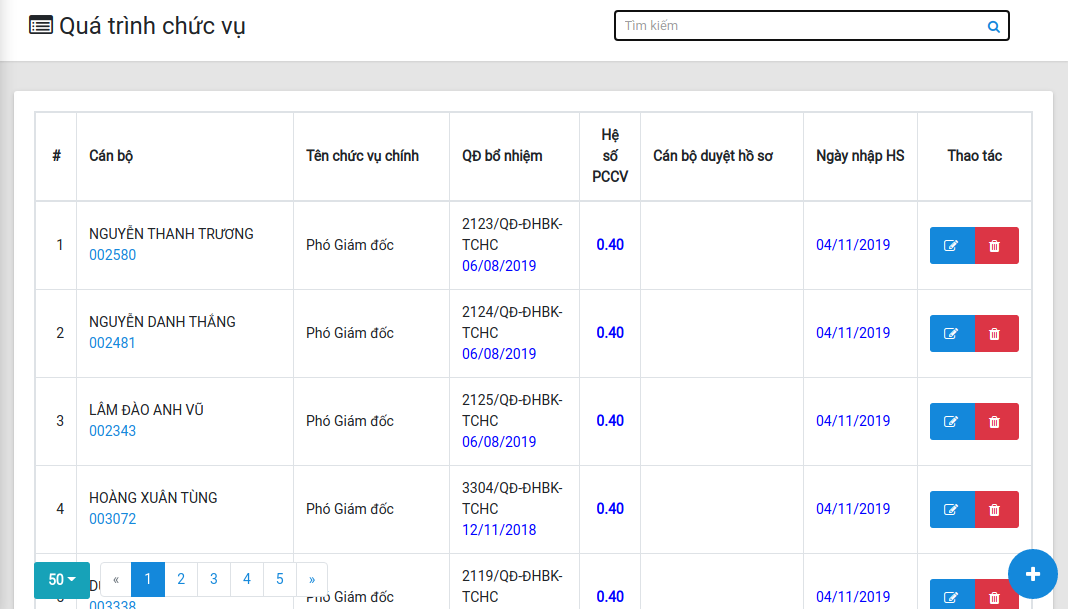
\includegraphics[scale=0.5]{img/Screen/qlquatrinh.png}
  \captionof{figure}{Quản lý quá trình chức vụ của cán bộ}
\end{center}
\textbf{Chức năng: Quản lý các tác vụ}\\
- Lược độ Activity:
\begin{center}
  \captionsetup{type=figure}
  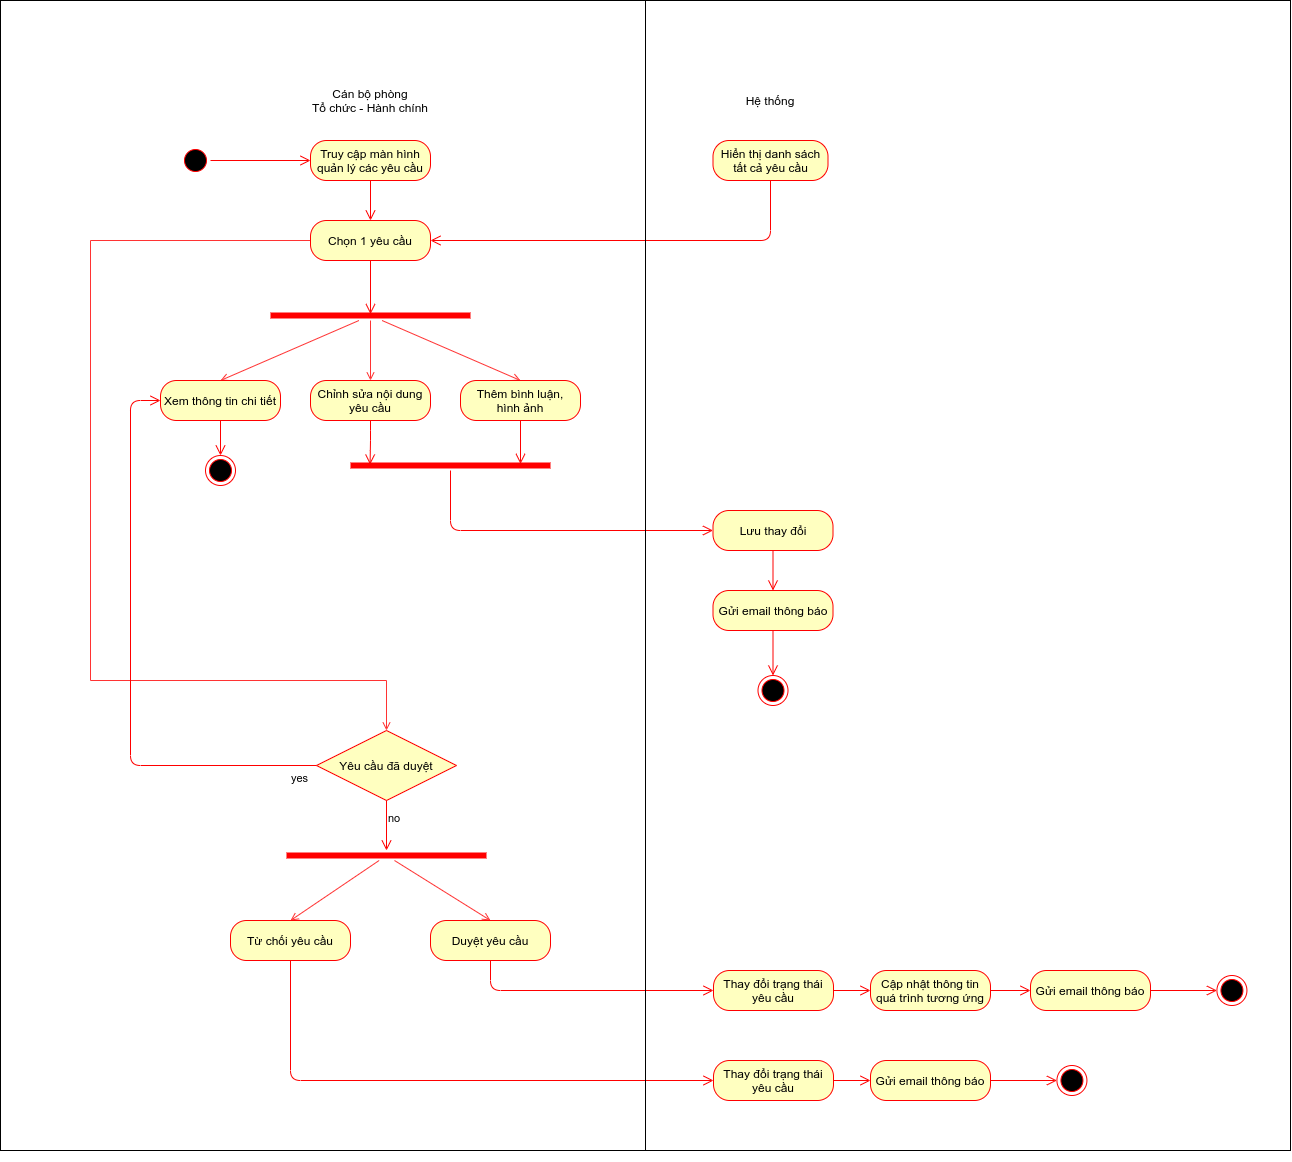
\includegraphics[scale=0.5]{img/UML/TchcStaff/activityQLTask.png}
  \captionof{figure}{Lược đồ Activity cho chức năng quản lý các yêu cầu của người dùng}
\end{center}
- Lược đồ Sequence:
- Hình ảnh chi tiết: 
\begin{center}
  \captionsetup{type=figure}
  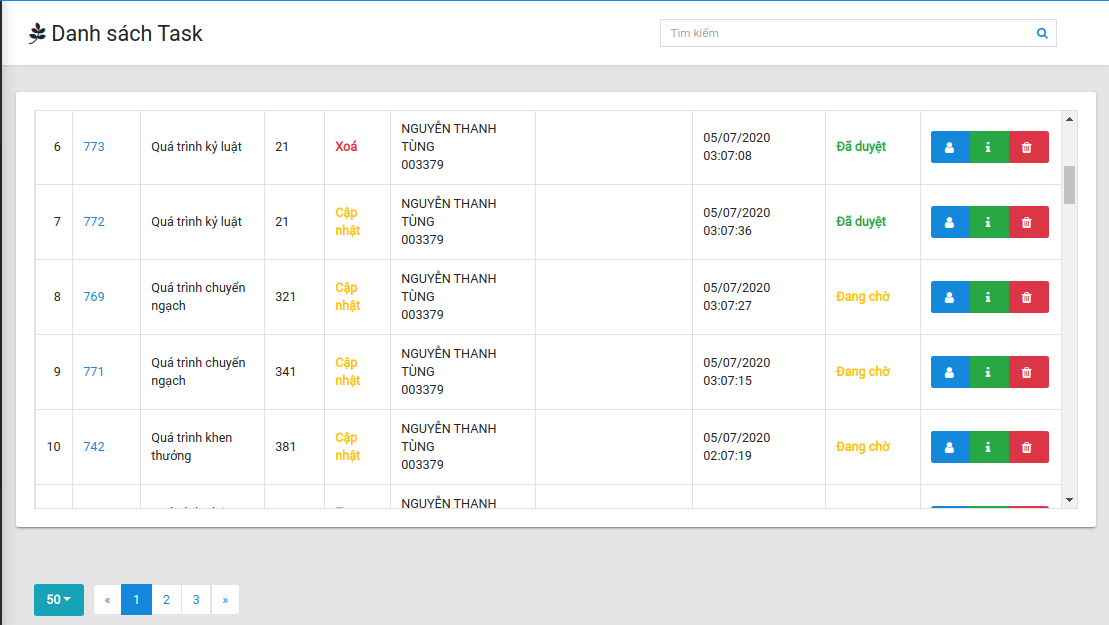
\includegraphics[scale=0.5]{img/Screen/qltask.png}
  \captionof{figure}{Xem toàn bộ yêu cầu của cán bộ}
\end{center}

\begin{center}
  \captionsetup{type=figure}
  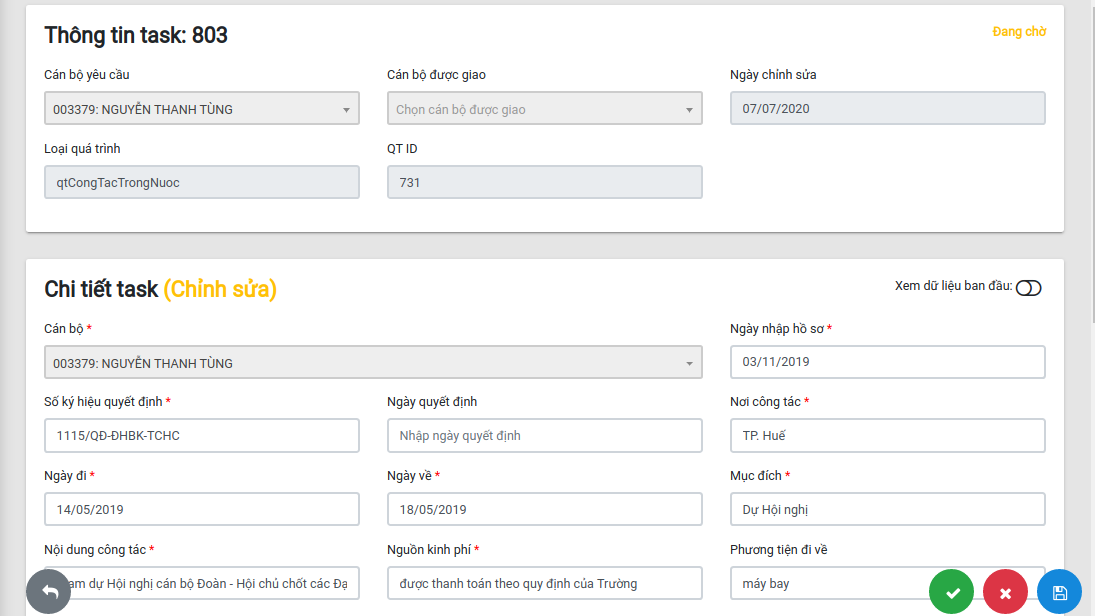
\includegraphics[scale=0.5]{img/Screen/chitiettask.png}
  \captionof{figure}{Xem thông tin chi tiết yêu cầu của cán bộ}
\end{center}
Khi xem chi tiết yêu cầu, cán bộ phòng Tổ chức - Hành chính có thể chỉnh sửa thông tin mà người dùng yêu cầu, sau đó đồng ý hoặc từ chứ duyệt yêu cầu. Bên cạnh đó cán bộ có thể để lại bình luận kèm theo những hình ảnh mình chứng (nếu có) cho yêu cầu.\\
\textbf{Chức năng: Giao các yêu cầu cần duyệt cho cán bộ phòng Tổ chức - Hành chính}\\
- Lược đồ Activity:
\begin{center}
  \captionsetup{type=figure}
  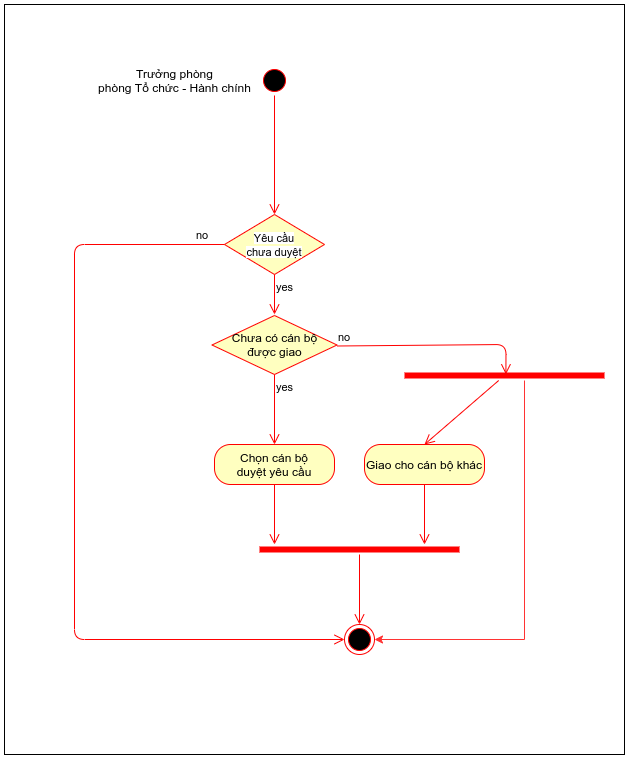
\includegraphics[scale=0.6]{img/UML/Manager/assignTask.png}
  \captionof{figure}{Lược đồ Activity cho chức năng giao yêu cầu cho cán bộ}
\end{center}
\subsection{Đối tượng: Người dùng}
\textbf{Chức năng: Quản lý thông tin}
\begin{center}
  \captionsetup{type=figure}
  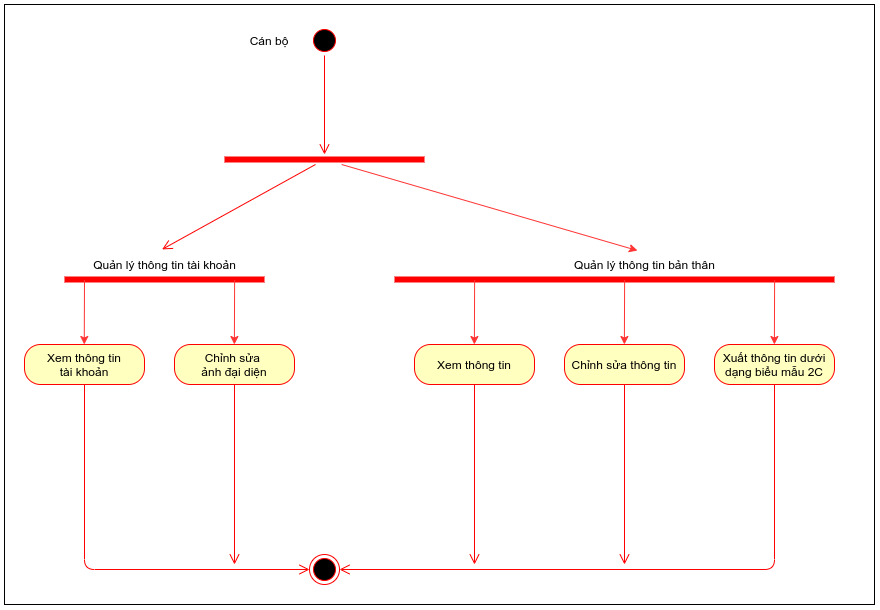
\includegraphics[scale=0.5]{img/UML/User/activityQLThongTin.png}
  \captionof{figure}{Lược đồ Activity cho chức năng quản lý thông tin cho cán bộ}
\end{center}
\textbf{Chức năng: Quản lý quá trình}
\begin{center}
  \captionsetup{type=figure}
  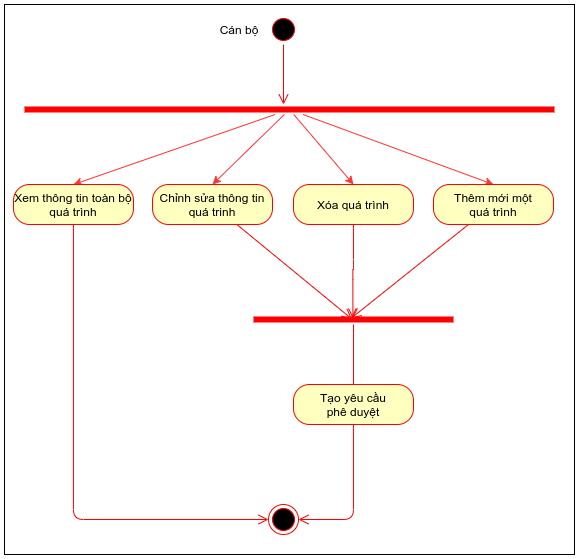
\includegraphics[scale=0.55]{img/UML/User/activityQuanLyQT.png}
  \captionof{figure}{Lược đồ Activity cho chức năng quản lý quá trình cho cán bộ}
\end{center}